
%\VignetteIndexEntry{Cardinal plotting}
%\VignettePackage{Cardinal}
%\VignetteEngine{utils::Sweave}
%\VignetteKeyword{Infrastructure, Proteomics, MassSpectrometry, IO}

\documentclass{article}

\RequirePackage{/Library/Frameworks/R.framework/Versions/3.1/Resources/library/BiocStyle/sty/Bioconductor}

\AtBeginDocument{\bibliographystyle{/Library/Frameworks/R.framework/Versions/3.1/Resources/library/BiocStyle/sty/unsrturl}}
\title{Cardinal plotting of ion images and mass spectra}

\author{Kyle D. Bemis}

\usepackage{Sweave}
\begin{document}
\Sconcordance{concordance:Cardinal-plotting.tex:Cardinal-plotting.Rnw:%
1 7 1 1 2 1 0 1 2 5 1 1 0 8 1 1 7 8 1 1 6 8 0 2 2 4 0 1 2 2 1 %
1 -4 1 8 3 1 1 2 1 0 1 2 4 0 2 2 4 0 2 2 1 0 2 1 3 0 1 2 4 1 %
1 2 4 0 1 3 4 0 1 2 3 1 1 -8 1 12 1 -9 1 13 4 1 1 2 4 0 1 3 4 %
0 1 2 3 1 1 -8 1 12 1 -9 1 13 4 1 1 2 4 0 1 2 2 1 1 -4 1 8 6 %
1 1 2 4 0 1 3 4 0 1 2 3 1 1 -8 1 12 1 -9 1 13 4 1 1 2 4 0 1 3 %
4 0 1 2 3 1 1 -8 1 12 1 -9 1 13 4 1 1 2 4 0 1 2 2 1 1 -4 1 8 %
5 1 1 2 11 0 1 2 1 1}


\maketitle

\tableofcontents

\section{Introduction}

One of the most important parts of working with mass spectrometry imaging datasets is visualization of the data by examining the ion images and mass spectra. \Rpackage{Cardinal} provides powerful functionality for plotting both ion images, mass spectra, as well as other representations of imaging data.

\section{Formula interface}

The plotting facilities of \Rpackage{Cardinal} are based on the powerful formula interface used by the \Robject{lattice} graphics package.

\section{Plotting using \Rpackage{Cardinal}}

For the following examples, we will use a simulated dataset. The image is a cardinal with red and black feathers, where the colors represent different regions of the image. The mass spectra will have two peaks to indicate the two regions. We use \Robject{generateImage} to generate the dataset from an integer matrix where $0$ represents black regions of the image and $1$ represents the red regions of the image.
\begin{Schunk}
\begin{Sinput}
> data <- matrix(c(NA, NA, 1, 1, NA, NA, NA, NA, NA, NA, 1, 1, NA, NA, 
+  NA, NA, NA, NA, NA, 0, 1, 1, NA, NA, NA, NA, NA, 1, 0, 0, 1, 
+  1, NA, NA, NA, NA, NA, 0, 1, 1, 1, 1, NA, NA, NA, NA, 0, 1, 1, 
+  1, 1, 1, NA, NA, NA, NA, 1, 1, 1, 1, 1, 1, 1, NA, NA, NA, 1, 
+  1, NA, NA, NA, NA, NA, NA, 1, 1, NA, NA, NA, NA, NA), nrow=9, ncol=9)
\end{Sinput}
\end{Schunk}
We can plot the ground truth image directly.
\begin{Schunk}
\begin{Sinput}
> image(data[,ncol(data):1], col=c("black", "red"))
\end{Sinput}
\end{Schunk}
\setkeys{Gin}{width=0.4\textwidth}
\begin{figure}
\begin{center}
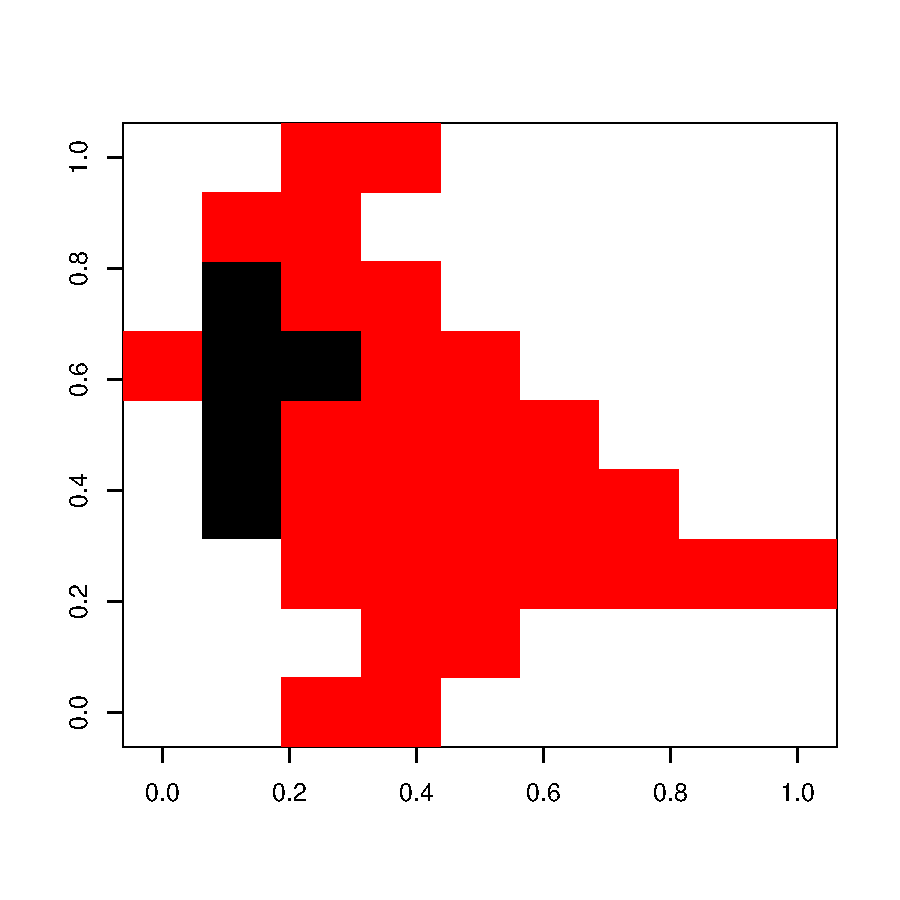
\includegraphics{Cardinal-plotting-005}
\caption{\small Ground truth image used to generate the simulated dataset.}
\end{center}
\end{figure}
Now we generate the data as if from a mass spectrometry imaging experiment with peaks at $m/z$ 3000 (higher intensity in black pixels) and $m/z$ 4000 (higher intensity in red pixels).
\begin{Schunk}
\begin{Sinput}
> set.seed(1)
> msset <- generateImage(data, range=c(1000,5000), centers=c(3000,4000), resolution=100,
+ 	step=3.3, as="MSImageSet")
\end{Sinput}
\end{Schunk}
We need to mark which pixels are black and which are red.
\begin{Schunk}
\begin{Sinput}
> pData(msset)$pg <- factor(data[is.finite(data)], labels=c("black", "red"))
\end{Sinput}
\end{Schunk}
Then we need to mark which features (which regions of the mass spectrum) belong to the peaks associated with ``black'' or ``red'' pixels; the rest of the spectrum is marked as background noise (\texttt{bg}).
\begin{Schunk}
\begin{Sinput}
> fData(msset)$fg <- factor(rep("bg", nrow(fData(msset))), levels=c("bg", "black", "red"))
> fData(msset)$fg[2950 < fData(msset)$mz & fData(msset)$mz < 3050] <- "black"
> fData(msset)$fg[3950 < fData(msset)$mz & fData(msset)$mz < 4050] <- "red"
\end{Sinput}
\end{Schunk}
Now we can experiment with different ways of plotting an imaging dataset.

\subsection{Plotting mass spectra}

The \verb|plot| method is used to plot mass spectra. The \Robject{pixel} argument is used to specify the pixel to use to plot the mass spectrum. If no conditioning is desired, the formula does not need to be specified explicitly.
\begin{Schunk}
\begin{Sinput}
> plot(msset, pixel=1)
\end{Sinput}
\end{Schunk}
\begin{Schunk}
\begin{Sinput}
> plot(msset, ~ mz, pixel=1)
\end{Sinput}
\end{Schunk}
\setkeys{Gin}{width=0.4\textwidth}
\begin{figure}
\begin{center}
\begin{tabular}{cc}
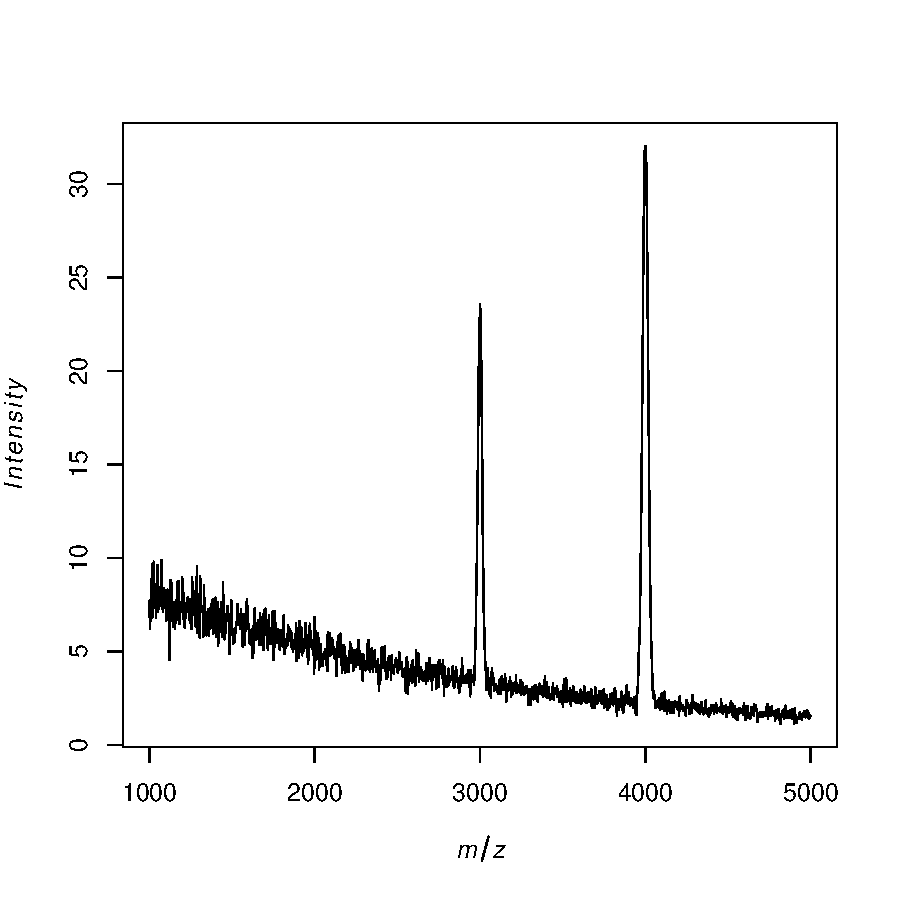
\includegraphics{Cardinal-plotting-011}
&
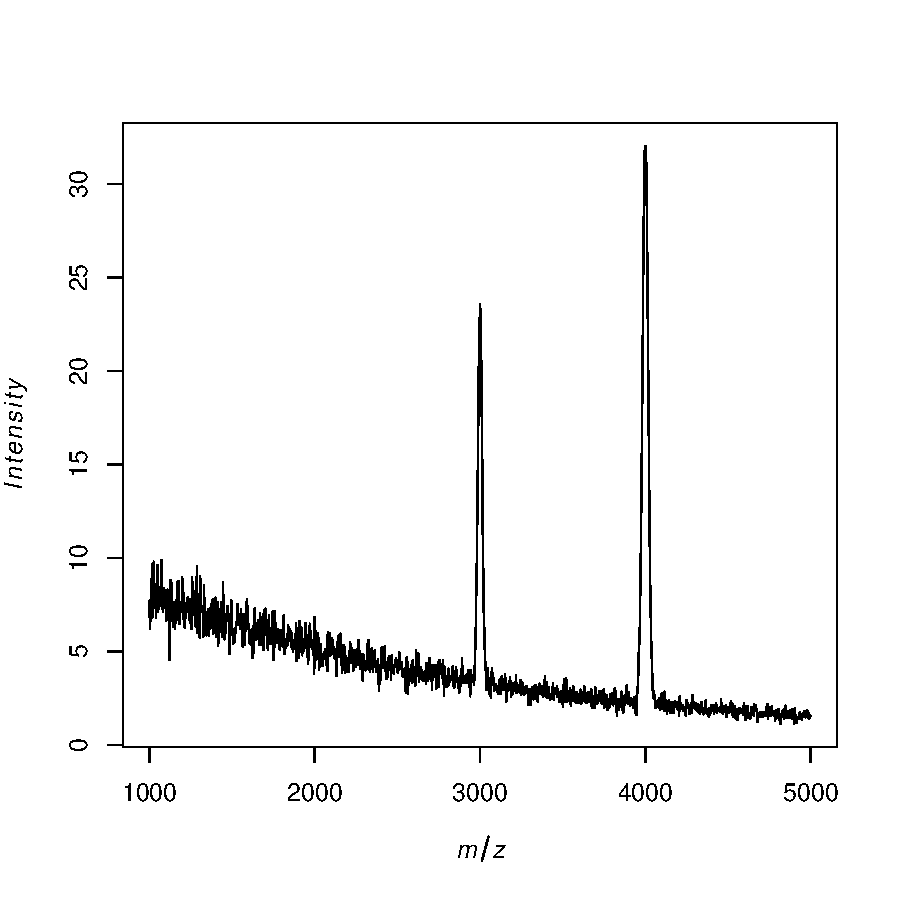
\includegraphics{Cardinal-plotting-012}
\end{tabular}
\caption{\small A simple mass spectrum plot. Both forms produce the same plot.}
\end{center}
\end{figure}
Specifying multiple pixels will apply a function, specified by \Robject{fun}, over those pixels. This can be used to create a plot of the mean spectrum (the default behavior). Below we obtain the mean spectrum of the red pixels, and the max spectrum of the black pixels.
\begin{Schunk}
\begin{Sinput}
> plot(msset, pixel=pData(msset)$pg=="red", fun=median, main="Median of red pixels")
\end{Sinput}
\end{Schunk}
\begin{Schunk}
\begin{Sinput}
> plot(msset, pixel=pData(msset)$pg=="black", fun=max, main="Max of black pixels")
\end{Sinput}
\end{Schunk}
\begin{figure}
\setkeys{Gin}{width=0.4\textwidth}
\begin{center}
\begin{tabular}{cc}
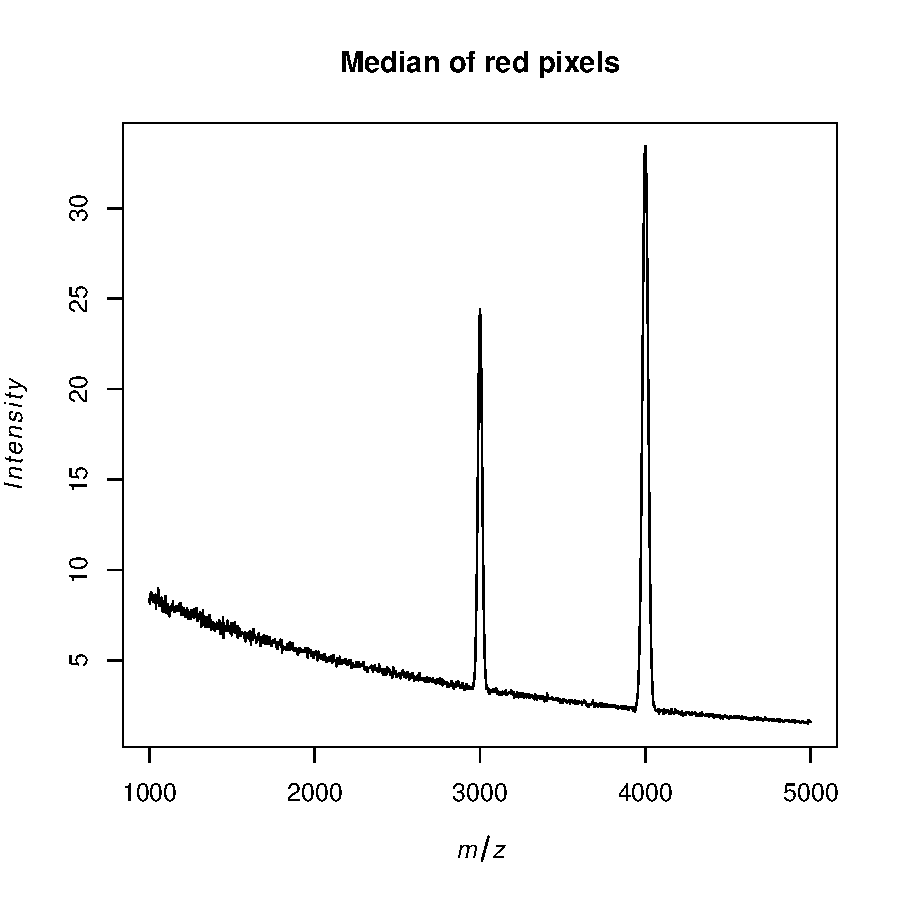
\includegraphics{Cardinal-plotting-015}
&
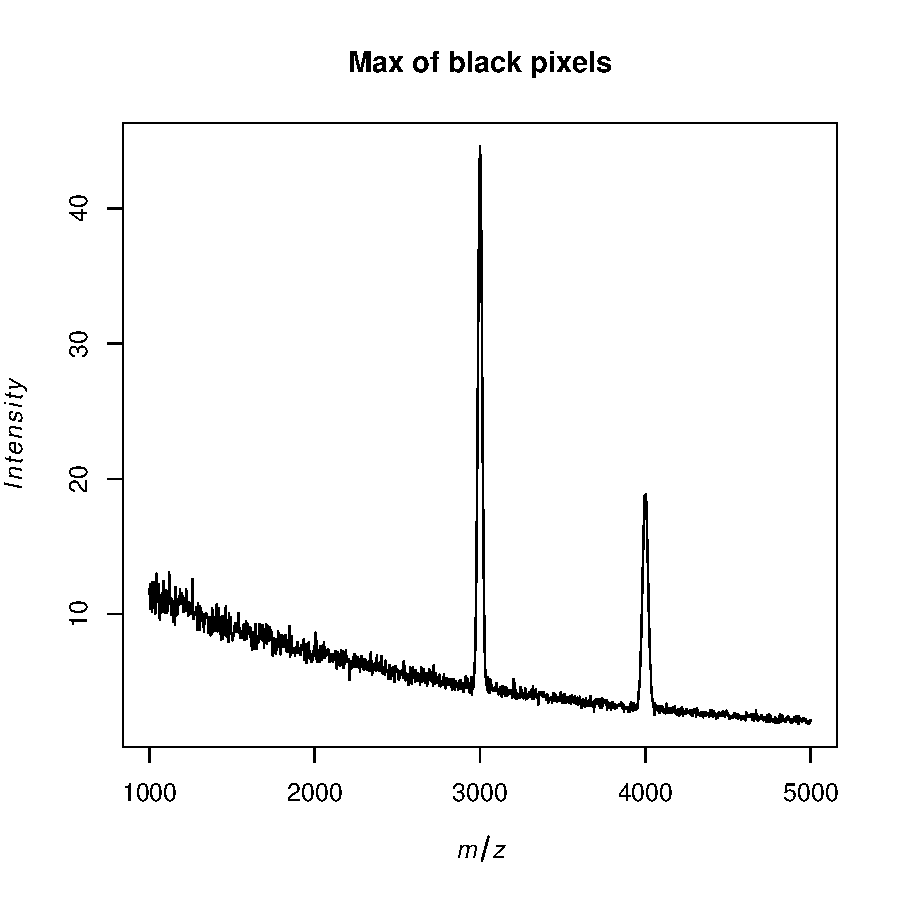
\includegraphics{Cardinal-plotting-016}
\end{tabular}
\caption{\small Applying a function over pixels to plot a median and max spectrum.}
\end{center}
\end{figure}
Using the \Robject{lattice} graphics option allows for more complex plots to be made. Conditioning on variables in the \Robject{formula} argument allows direct comparison between regions of the image or mass spectrum. For example, by conditioning on the variable \verb|pData(msset)$pg| which specifies the color of the pixels, we can obtain mean spectra for each type of pixel in a single step; notice that the \verb|plot| method knows where to find the \Robject{pg} variable, because it is contained in \Robject{msset}. Likewise, we use the \Robject{fg} variable (which we used to mark notable $m/z$-values) with the argument \Robject{groups} to distinguish different regions of the mass spectrum with different colors.
\begin{Schunk}
\begin{Sinput}
> print(plot(msset, ~ mz | pg, pixel=1:ncol(msset), groups=fg, lattice=TRUE, col=c("blue", "black", "red")))
\end{Sinput}
\end{Schunk}
\begin{figure}
\setkeys{Gin}{width=0.8\textwidth}
\begin{center}
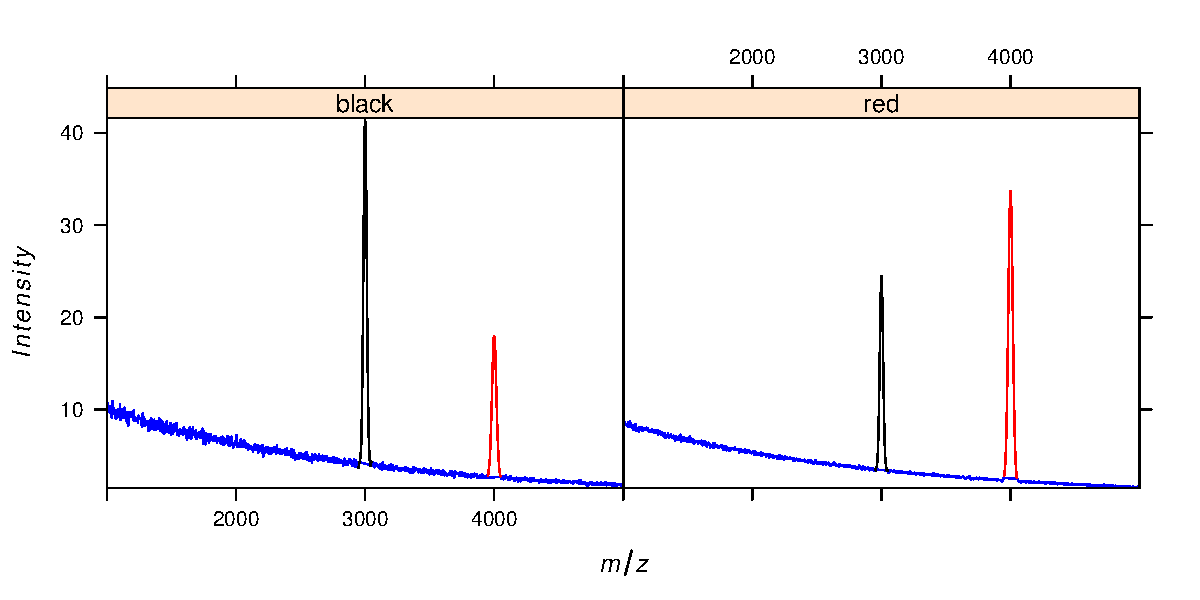
\includegraphics{Cardinal-plotting-018}
\caption{\small A plot conditioning on variables using \Robject{lattice} graphics.}
\end{center}
\end{figure}

\subsection{Plotting ion images}

The \verb|image| method is used to plot images. The \Robject{feature} argument is used to specify the feature to use to create the image. For a mass spectrometry imaging dataset, the features are the $m/z$-values corresponding to single-ion images. As before, if no conditioning is desired, the formula does not need to be specified explicitly.
\begin{Schunk}
\begin{Sinput}
> image(msset, feature=1, col.regions=gradient.colors(100, "red", "black"))
\end{Sinput}
\end{Schunk}
\begin{Schunk}
\begin{Sinput}
> image(msset, ~ x * y, feature=1, col.regions=gradient.colors(100, "red", "black"))
\end{Sinput}
\end{Schunk}
\begin{figure}
\setkeys{Gin}{width=0.4\textwidth}
\begin{center}
\begin{tabular}{cc}
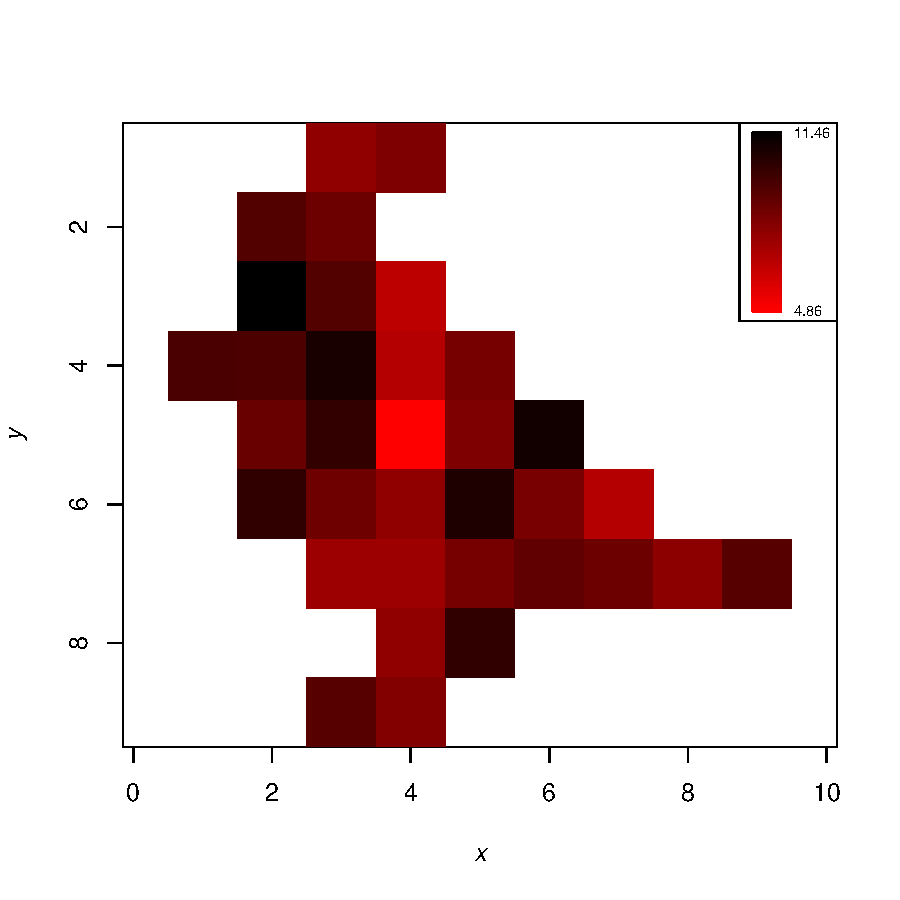
\includegraphics{Cardinal-plotting-021}
&
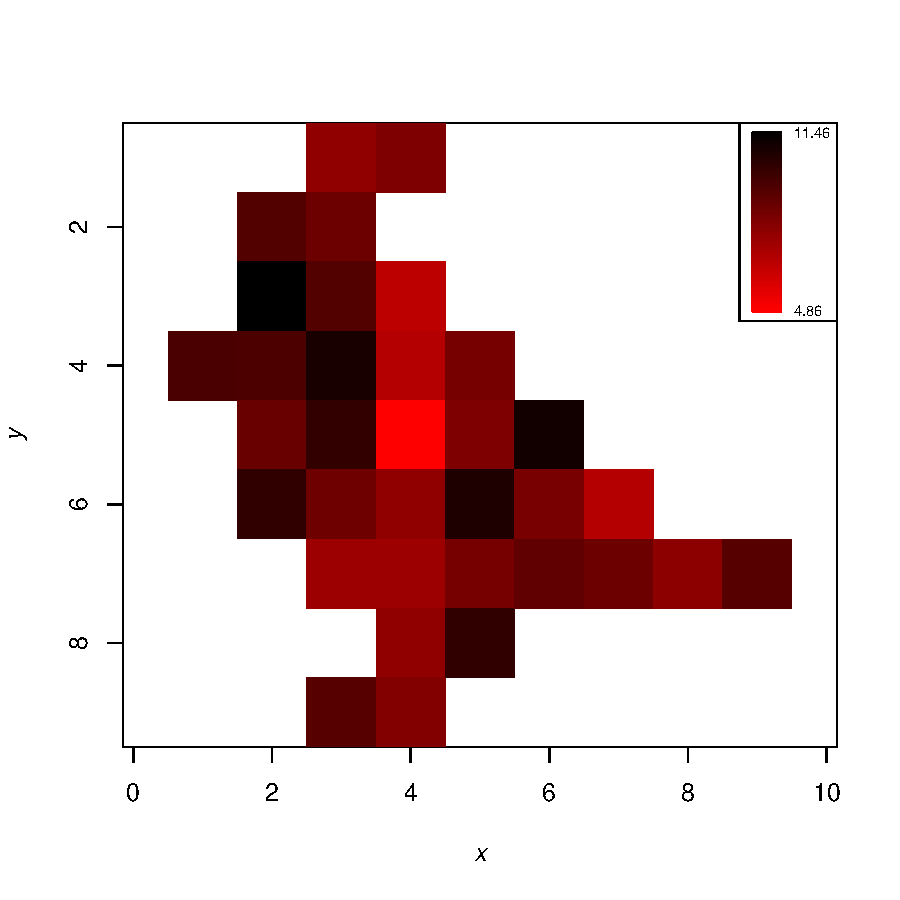
\includegraphics{Cardinal-plotting-022}
\end{tabular}
\caption{\small A simple single-ion image. Both forms produce the same plot.}
\end{center}
\end{figure}
Like with the \verb|plot| method, the \verb|image| method can apply functions over features ($m/z$-values) when multiple features are specified. By default, \verb|mean| is used to average the images over the features. In the following example, we specify two plots, first using the features from the peak that has a higher intensity associated with black pixels, and then using the features from the peak that has a higher intensity associated with red pixels.
\begin{Schunk}
\begin{Sinput}
> image(msset, feature=fData(msset)$fg=="black", col.regions=alpha.colors(100, "black"))
\end{Sinput}
\end{Schunk}
\begin{Schunk}
\begin{Sinput}
> image(msset, feature=fData(msset)$fg=="red", col.regions=alpha.colors(100, "red"))
\end{Sinput}
\end{Schunk}
\begin{figure}
\setkeys{Gin}{width=0.4\textwidth}
\begin{center}
\begin{tabular}{cc}
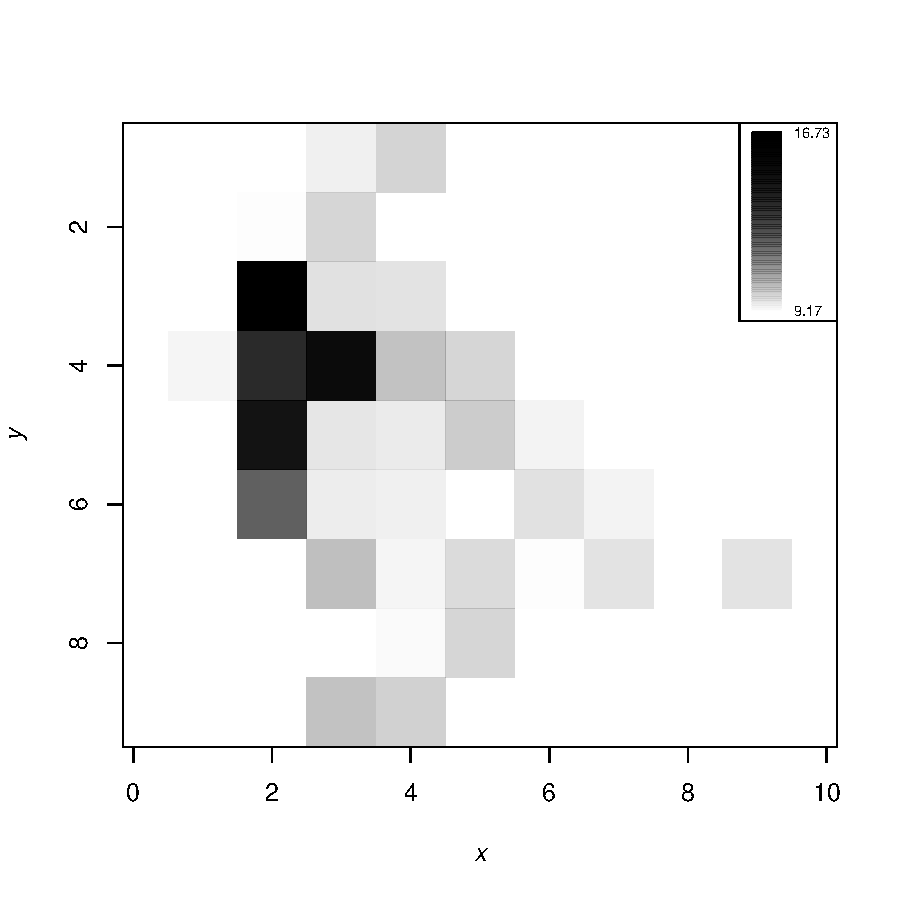
\includegraphics{Cardinal-plotting-025}
&
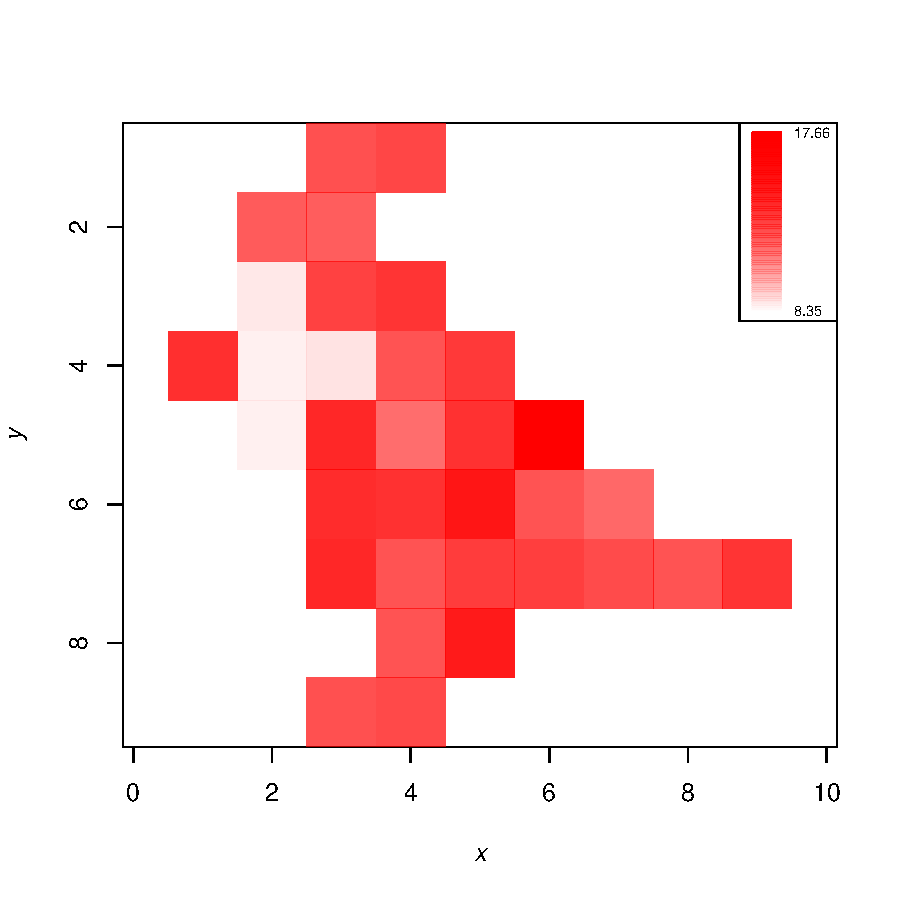
\includegraphics{Cardinal-plotting-026}
\end{tabular}
\caption{\small Averaging over different sets of mass features.}
\end{center}
\end{figure}
Using a \Robject{lattice}-style formula, we can condition on other variables with \verb|image| too. Here we use all of the features, but condition on which part of the mass spectrum those features come from using the variable \verb|fData(msset)$fg|. Again, since \verb|image| knows to look in \Robject{msset}, we only need to specify the variable as \Robject{fg}.
\begin{Schunk}
\begin{Sinput}
> print(image(msset, ~ x * y | fg, feature=1:nrow(msset), col.regions=intensity.colors(100), lattice=TRUE))
\end{Sinput}
\end{Schunk}
\begin{figure}
\setkeys{Gin}{width=0.8\textwidth}
\begin{center}
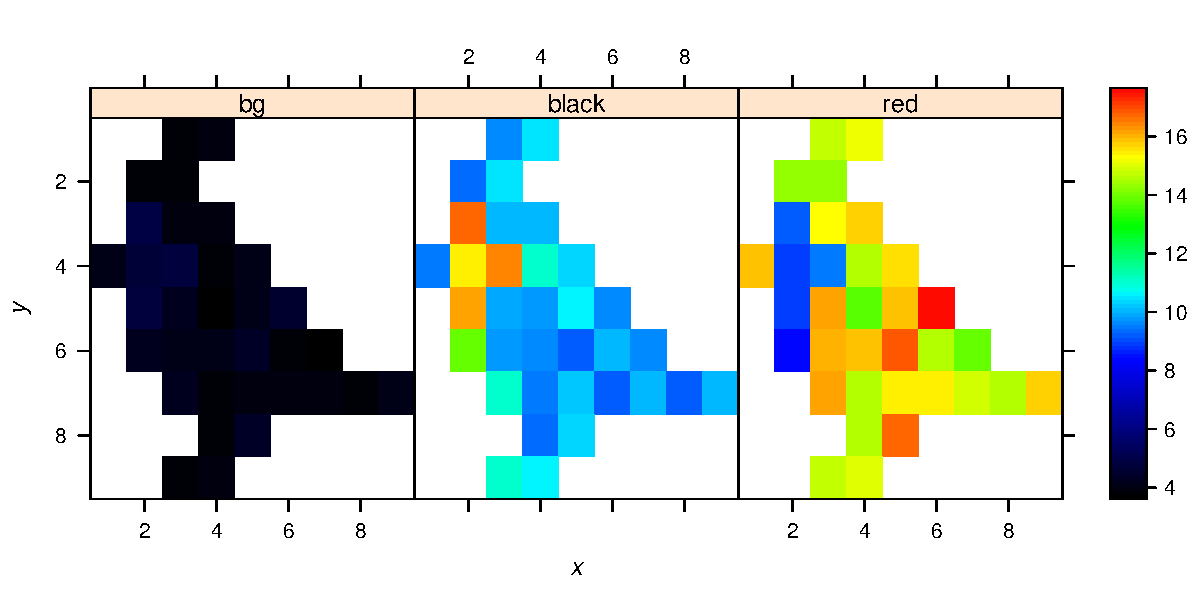
\includegraphics{Cardinal-plotting-028}
\caption{\small Images conditioning on variables using \Robject{lattice} graphics.}
\end{center}
\end{figure}

\section{Session info}

\begin{itemize}\raggedright
  \item R version 3.1.1 (2014-07-10), \verb|x86_64-apple-darwin13.1.0|
  \item Locale: \verb|en_US.UTF-8/en_US.UTF-8/en_US.UTF-8/C/en_US.UTF-8/en_US.UTF-8|
  \item Base packages: base, datasets, graphics, grDevices,
    methods, parallel, stats, utils
  \item Other packages: Biobase~2.24.0, BiocGenerics~0.10.0,
    Cardinal~0.8.2
  \item Loaded via a namespace (and not attached):
    BiocStyle~1.2.0, fields~7.1, grid~3.1.1, irlba~1.0.3,
    lattice~0.20-29, maps~2.3-7, MASS~7.3-33, Matrix~1.1-4,
    signal~0.7-4, sp~1.0-15, spam~0.41-0, stats4~3.1.1,
    tools~3.1.1
\end{itemize}
\end{document}
